\section{Simulation Analysis}
\label{sec:simulation}

In this section, Ngspice was used in order to simulate the AC/DC converter. Some modifications were made from the original circuit in order of simplification. First of all, the transformer was replaced by an ideal using a depedent current source (instead of the primary) and a dependent voltage source (instead of the secundary) and this allowed us to not having to model a real transformer.\\
Then, the values of n (parameter of dependency sources), the C (capacitance) of the capacitor
and the values of the resistance of the resistors were being adjusted through trial and error in order to achieve
the maximum accurary of the output voltage, since the initial goal was to get this value close as possible to 12 V.

\subsection{Second sector: Envelope detector circuit (rectifier + capacitor)}

Then we go to the second sector, analysing in NGspice
 comparation with Octave is clear in figures x e y.

This next table represents the Ngspice results for the output of the envelope.

 \begin{table}[H] \centering
\begin{tabular}{|
>{\columncolor[HTML]{FFCC67}}l |c|}
\hline
\multicolumn{2}{|l|}{\cellcolor[HTML]{EABD8B}Name - Value} \\ \hline
maximum(v(4))-minimum(v(4)) & 1.447754e-01\\ \hline
mean(v(4)) & 1.946163e+01\\ \hline

\end{tabular}
\caption{Results for the output of the envelope}
\end{table}

After analysis of the tables above, some discrepancies are observed. Nevertheless, these are due to the
osilations that naturally occur in ngspice. These happen because the diodes used are non-linear components,
which means that a linear relaton between the current and the voltage does not exist. The exponential function
that comes into the equations leads to these type of oscilation.

\begin{figure}[H] 
\centering
\begin{subfigure}{0.4\textwidth}
\includegraphics[width=\textwidth]{MainPlot.eps}
\caption{Octave}
\label{fig:first}
\end{subfigure}
\begin{subfigure}{0.3\textwidth}
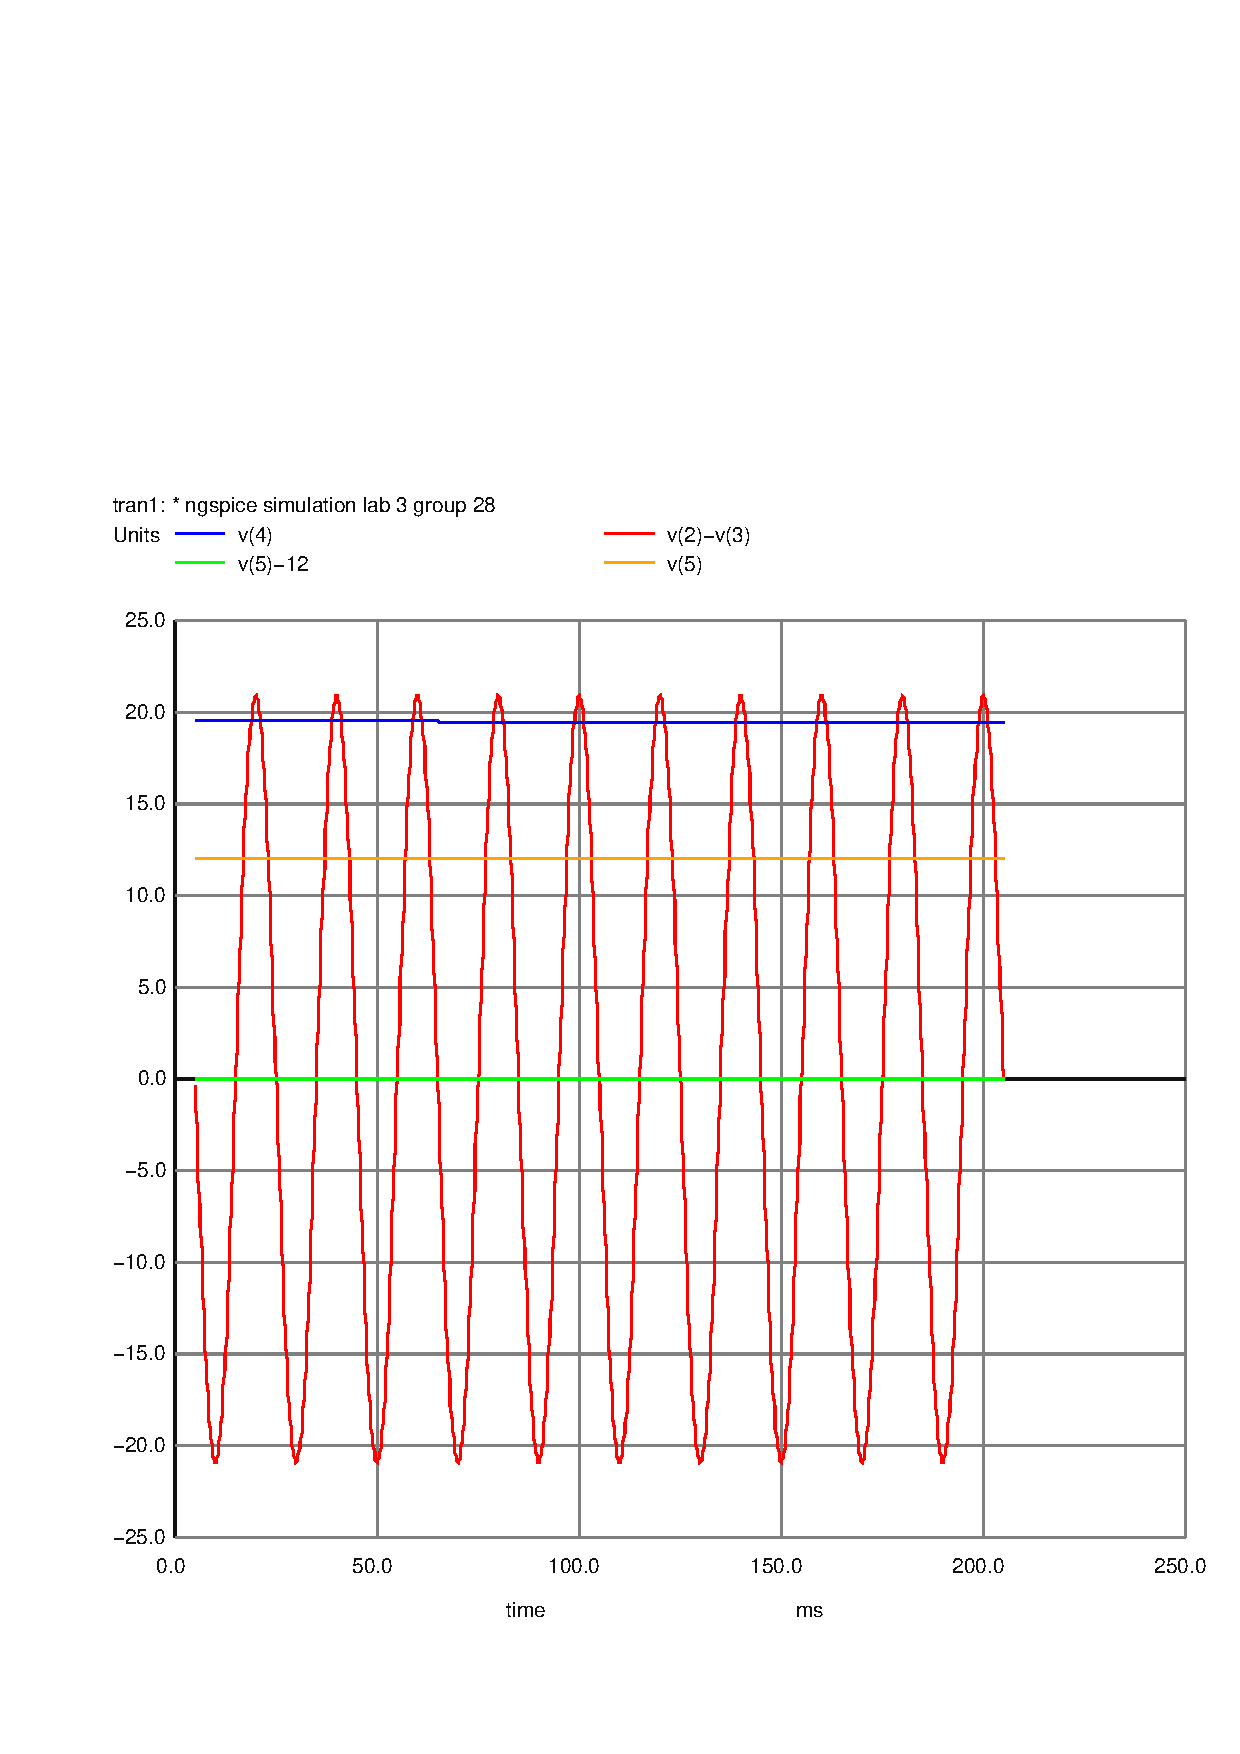
\includegraphics[width=\textwidth]{sim3.pdf}
\caption{NGSPICE}
\label{fig:second}
\end{subfigure}
\caption{Input voltage of the secundary circuit (v(2)), output Voltage of the Envelope Detector (v(4)), Voltage
Regulator (v(5)), and v(5)-12}
\end{figure}

\subsection{Third sector: Voltage regulator circuit}

Then we go to the third sector, analysing in NGspice
 comparation with Octave is clear in figures x e y.
 
 
This next table represents the Ngspice results for the voltage regulator.
 
 \begin{table}[H] \centering
\begin{tabular}{|
>{\columncolor[HTML]{FFCC67}}l |c|}
\hline
\multicolumn{2}{|l|}{\cellcolor[HTML]{EABD8B}Name - Value} \\ \hline
@gb[i] & 0.000000e+00\\ \hline
@r1[i] & 0.000000e+00\\ \hline
@r2[i] & 0.000000e+00\\ \hline
@r3[i] & 0.000000e+00\\ \hline
@r4[i] & 0.000000e+00\\ \hline
@r5[i] & -1.63724e-02\\ \hline
@r6[i] & 0.000000e+00\\ \hline
@r7[i] & 0.000000e+00\\ \hline
v(1) & 0.000000e+00\\ \hline
v(2) & 0.000000e+00\\ \hline
v(3) & 0.000000e+00\\ \hline
v(5) & 0.000000e+00\\ \hline
v(6) & 5.000000e+01\\ \hline
v(7) & 0.000000e+00\\ \hline
v(8) & 0.000000e+00\\ \hline
v(9) & 0.000000e+00\\ \hline

\end{tabular}
\caption{Results for the voltage regulator}
\end{table}
 
 
 The oscilations between theorectial and simulation results that happened in the output voltage of the envelope detector are extended to the voltage regulator for the same reasons. Therefore, it was expected to happen a small discrepancy between the results of both models. Nevertheless, we believe that once theoutput voltage is aproximately 12V, as wanted, the model worked successfuly.\\
 The implemented circuit gave us a MERIT of 0.36 in NGSpice and 11.68 in Octave. 

%SO TEMOS DUAS FIGURAS PARA IMPRIMIR NO NGSPICE, como coloca-las, final, ou em cada subsection
\begin{figure}[H] 
\centering
\begin{subfigure}{0.4\textwidth}
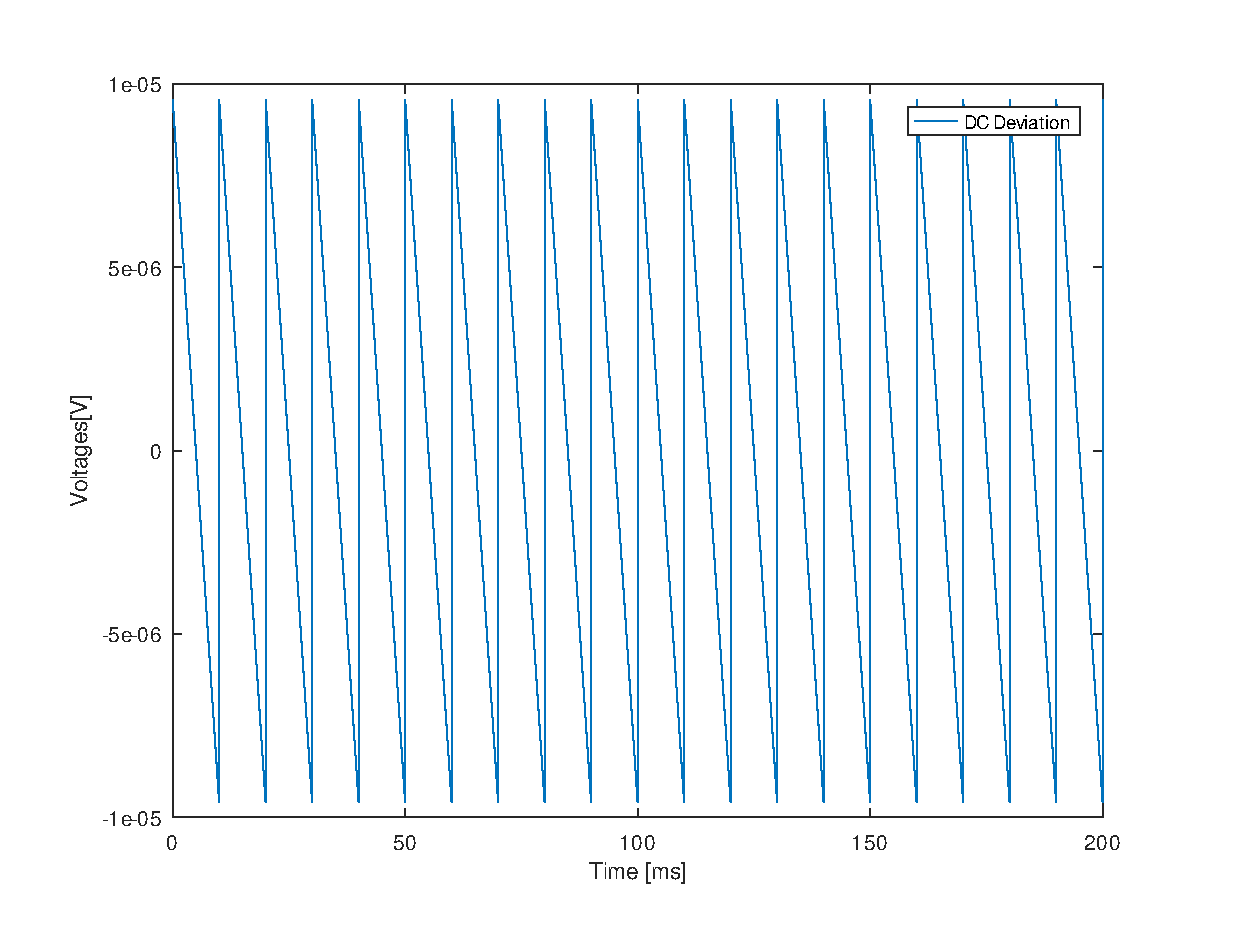
\includegraphics[width=\textwidth]{DCDeviation.eps}
\caption{Octave}
\label{fig:first}
\end{subfigure}
\begin{subfigure}{0.3\textwidth}
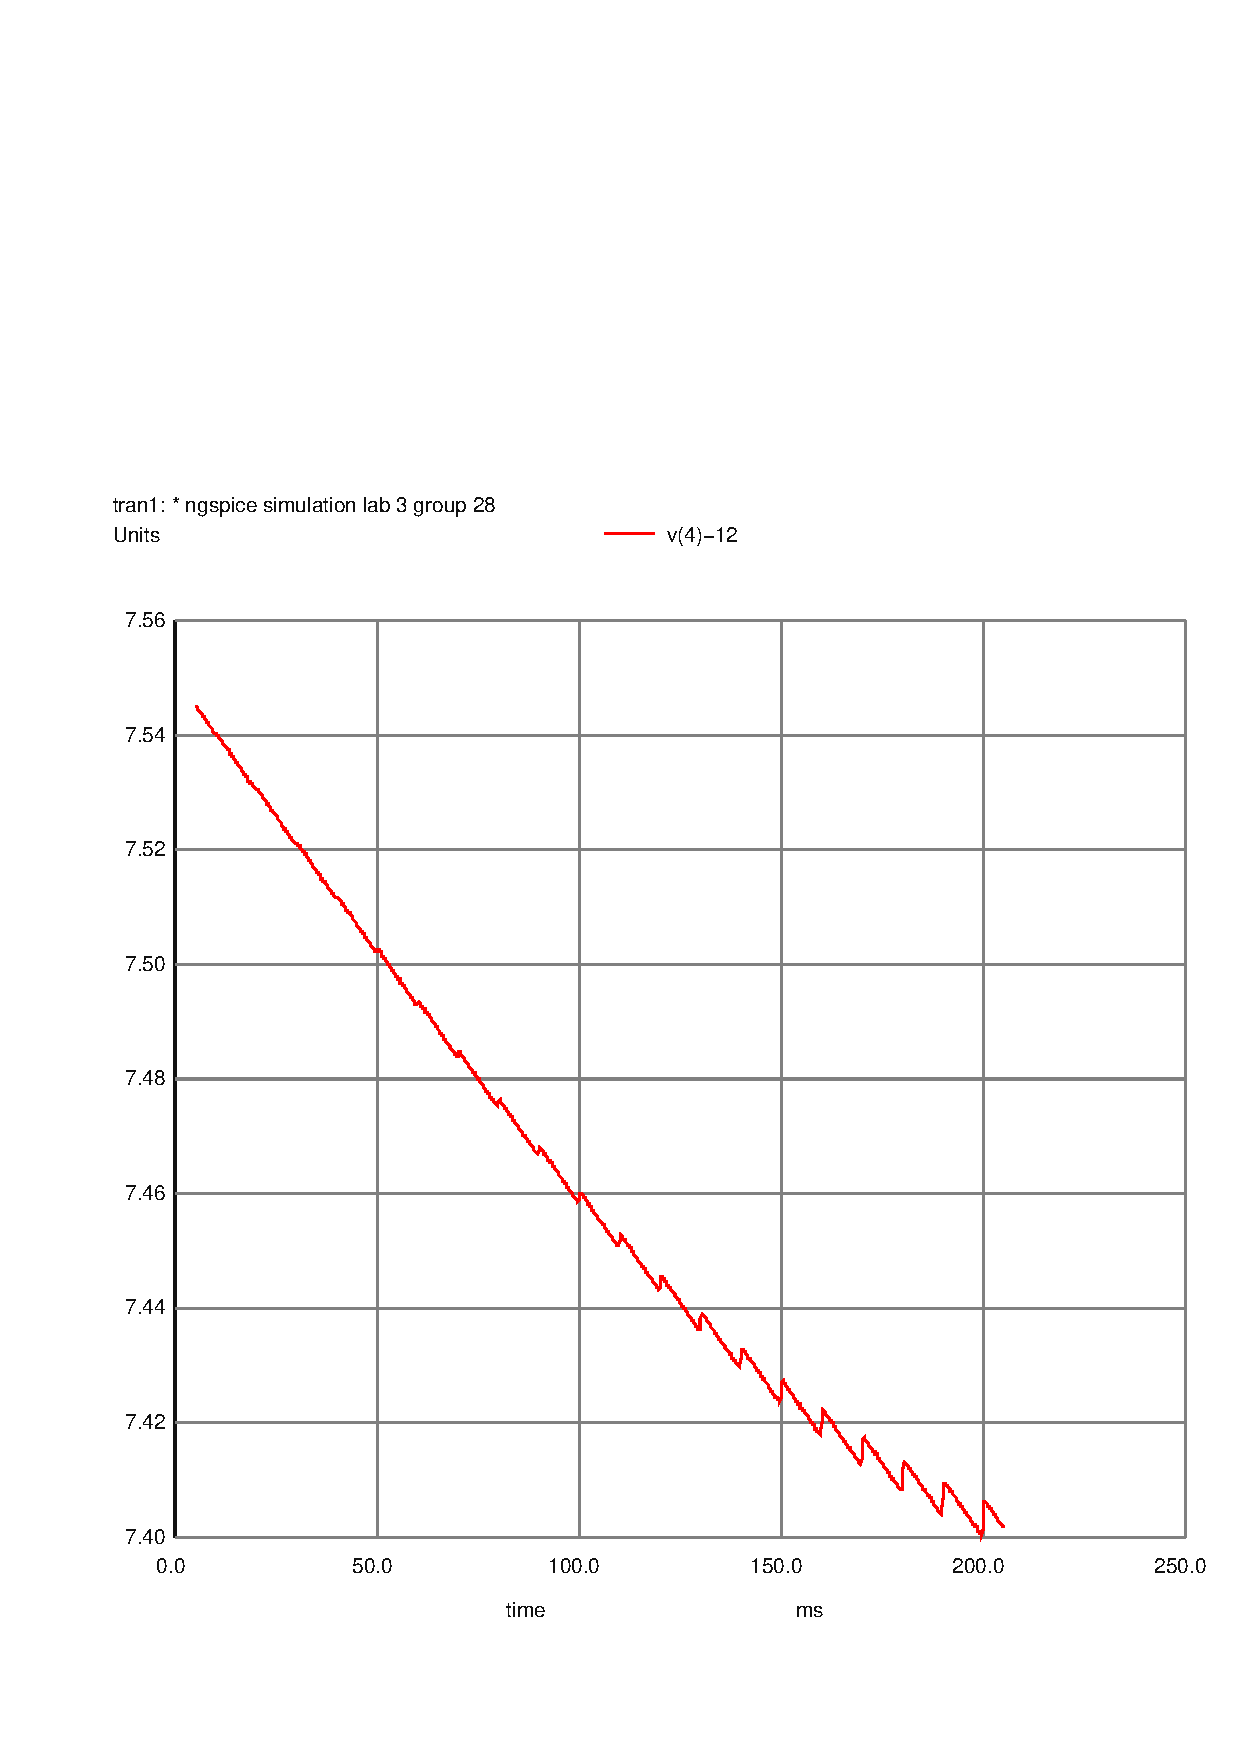
\includegraphics[width=\textwidth]{sim31.pdf}
\caption{NgSpice}
\label{fig:second}
\end{subfigure}
\caption{Output DC Deviation}
\end{figure}

\begin{figure}[H] 
\centering
\begin{subfigure}{0.4\textwidth}
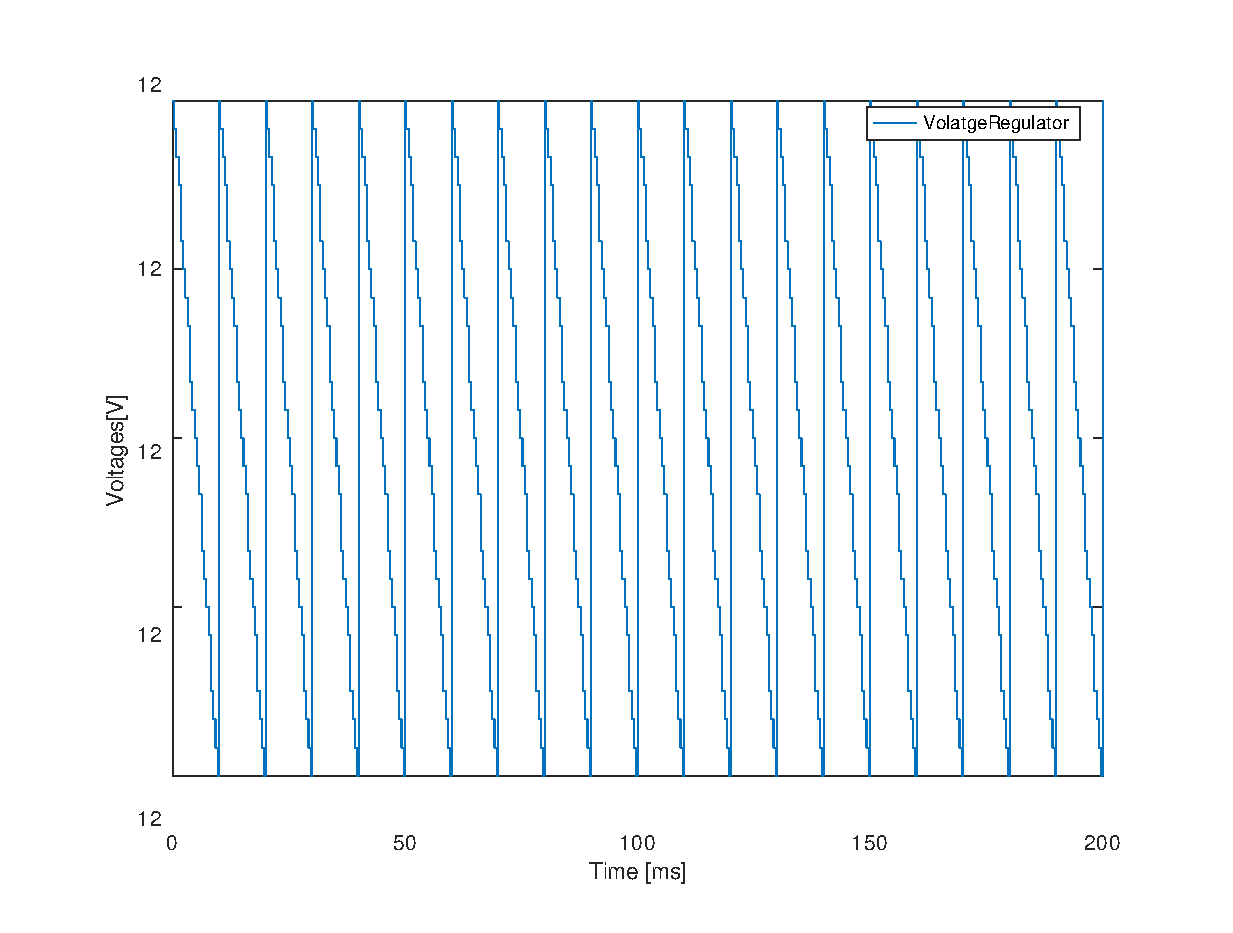
\includegraphics[width=\textwidth]{VoltageRegulator.eps}
\caption{Octave}
\label{fig:first}
\end{subfigure}
\begin{subfigure}{0.3\textwidth}
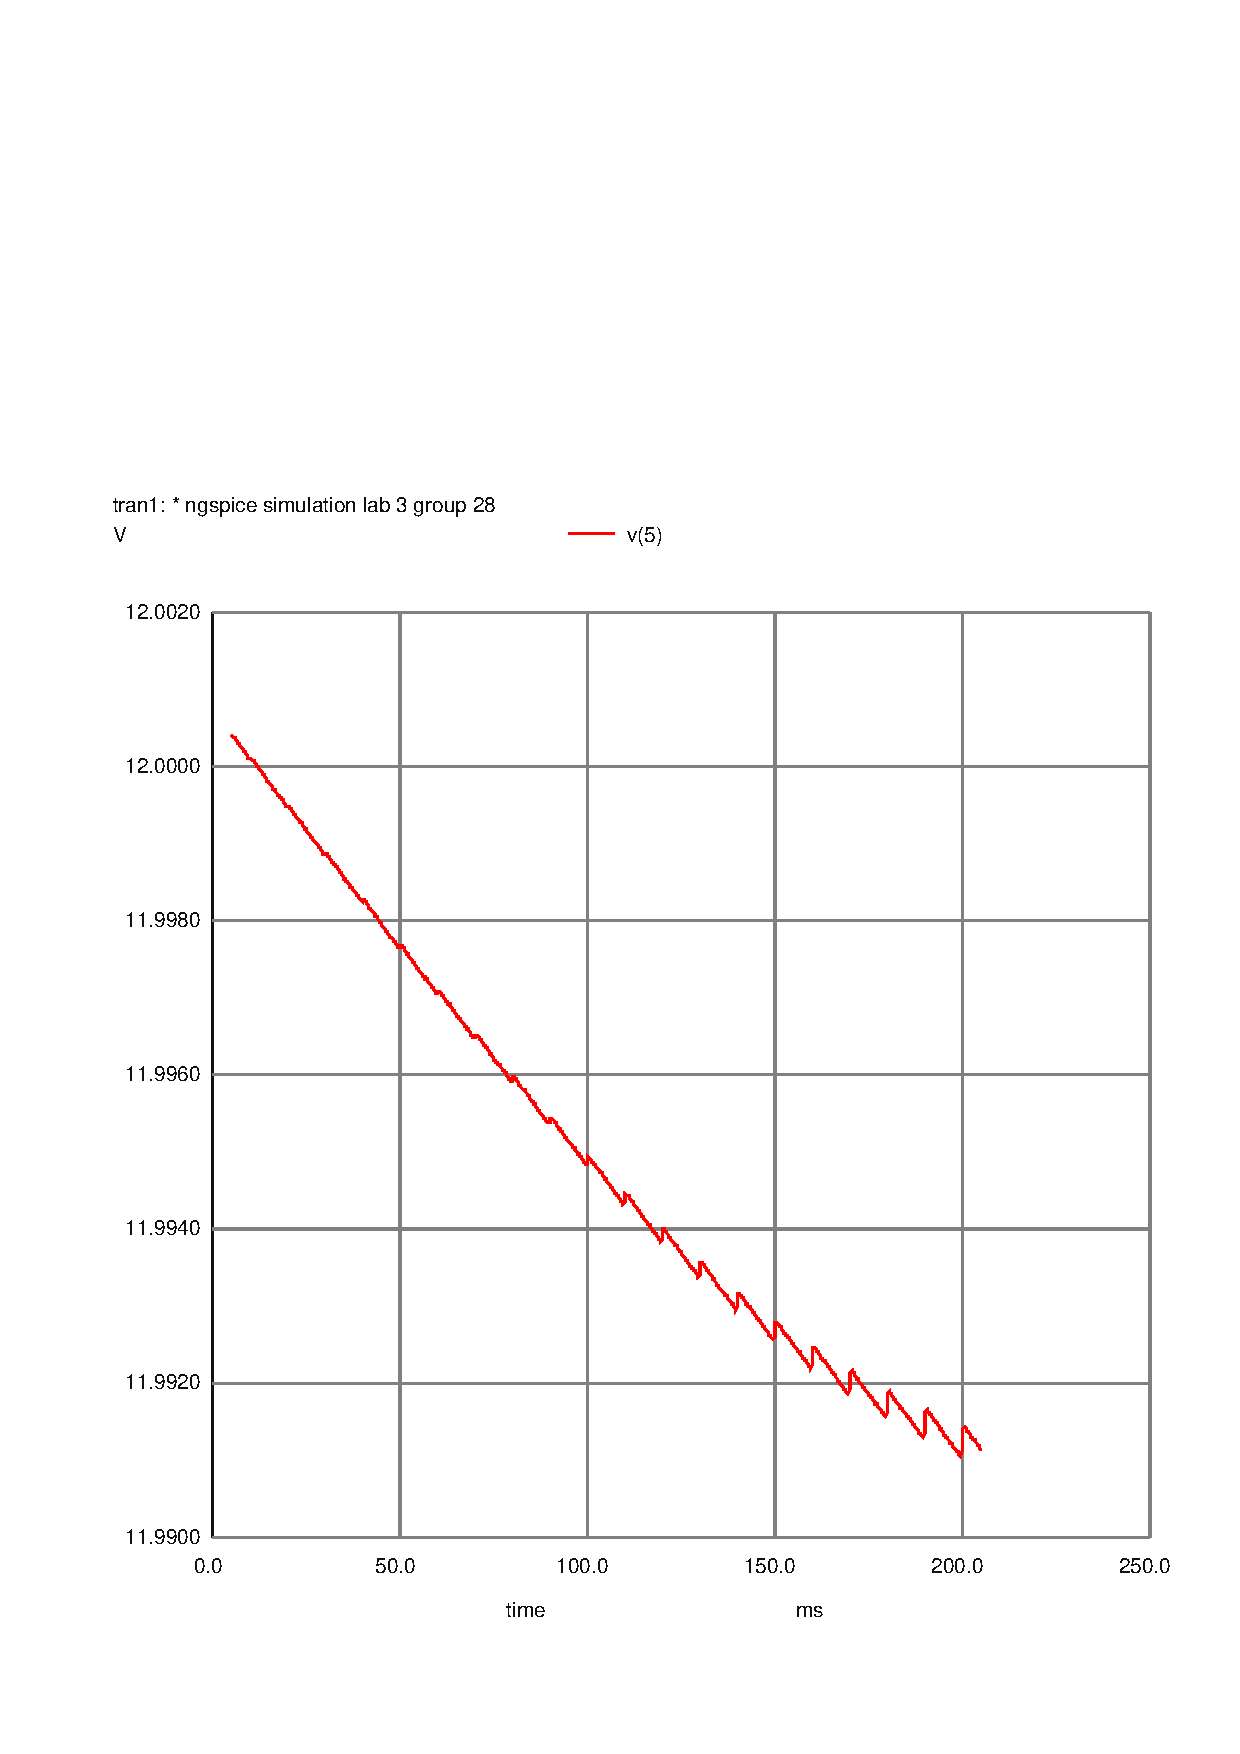
\includegraphics[width=\textwidth]{sim33.pdf}
\caption{NGSPICE}
\label{fig:second}
\end{subfigure}
\caption{Output Voltage}
\end{figure}
